\chapter{Déploiement et DevOps}


\chapteropeningtext{Après l'implémentation des différentes parties de SomaScan, ce chapitre présente l'environnement de production et les pratiques DevOps mises en place pour livrer la solution. Il décrit l'infrastructure utilisée, le processus de déploiement du backend Laravel et de l'application web React, le mode de distribution de l'application mobile Flutter, ainsi que l'organisation du code source autour de GitHub et des pipelines de déploiement.\par\medskip L'objectif de ce chapitre est de montrer comment la solution passe d'un environnement de développement local à un environnement exploitable en production. Il met également en évidence les mesures de sécurité, le processus de livraison automatisé et les limites actuelles de l'infrastructure, notamment l'absence d'une stratégie de sauvegarde automatisée de la base de données.}{Déploiement -- ValaBlue -- GitHub Actions -- CI/CD -- Sécurité -- Limites}

\section{Environnement de production et architecture de déploiement}

La solution est déployée sur l'infrastructure d'hébergement ValaBlue, un prestataire marocain proposant des services d'hébergement web. L'environnement utilisé correspond à une plateforme d'hébergement mutualisé administrée à travers cPanel. Cette plateforme permet d'héberger à la fois des applications PHP et des sites web statiques, ce qui permet de regrouper le backend Laravel et l'application web React sur la même infrastructure.

Les accès disponibles pour l'administration et le déploiement sont les suivants :

\begin{itemize}
    \item accès cPanel pour la gestion générale de l'hébergement ;
    \item accès SSH pour l'exécution des commandes de déploiement ;
    \item accès Git pour la mise à jour du code source sur le serveur ;
    \item accès aux fichiers générés du frontend après compilation.
\end{itemize}

Le tableau~\ref{tab:environnement-production} synthétise les principaux éléments de l'environnement de production.

\begin{table}[H]
\centering
\begin{tabularx}{\textwidth}{|p{4.2cm}|X|}
\hline
\textbf{Élément} & \textbf{Description} \\
\hline
Hébergement & Plateforme mutualisée ValaBlue administrée avec cPanel et accessible par SSH. \\
\hline
Backend & Application Laravel déployée sur le même serveur, avec Nginx, PHP 8.2 et Composer. \\
\hline
Frontend web & Application React compilée puis déployée sous forme de fichiers statiques sur le serveur. \\
\hline
Base de données & Base de données fournie par le même hébergeur, avec un espace alloué de 5~Go. \\
\hline
Mobile & Application Flutter installée manuellement sur les appareils Android fournis par l'entreprise. \\
\hline
Sécurité réseau & Domaines et sous-domaines de production protégés par des certificats SSL valides. \\
\hline
\end{tabularx}
\caption{Environnement de production de SomaScan}
\label{tab:environnement-production}
\end{table}

Le backend Laravel expose les API publiques utilisées par l'application mobile et par l'application web. L'application web React est déployée sur le même serveur et communique avec le backend à travers l'URL de l'API de production. L'application mobile, quant à elle, est installée sur des téléphones Android administrés par l'entreprise et communique directement avec les endpoints publics du backend.

Le routage de l'application web utilise un mode basé sur le hash, par exemple \texttt{\#/dashboard}. Ce choix simplifie le déploiement sur un hébergement statique ou mutualisé, car il évite d'exiger une configuration serveur avancée pour rediriger toutes les routes vers le fichier \texttt{index.html}.

Le backend ne nécessite actuellement aucun cron job. Les traitements sont déclenchés par les requêtes API, notamment les scans envoyés depuis l'application mobile, les actions d'administration et les demandes de reporting depuis l'application web.

\begin{figure}[H]
    \centering
    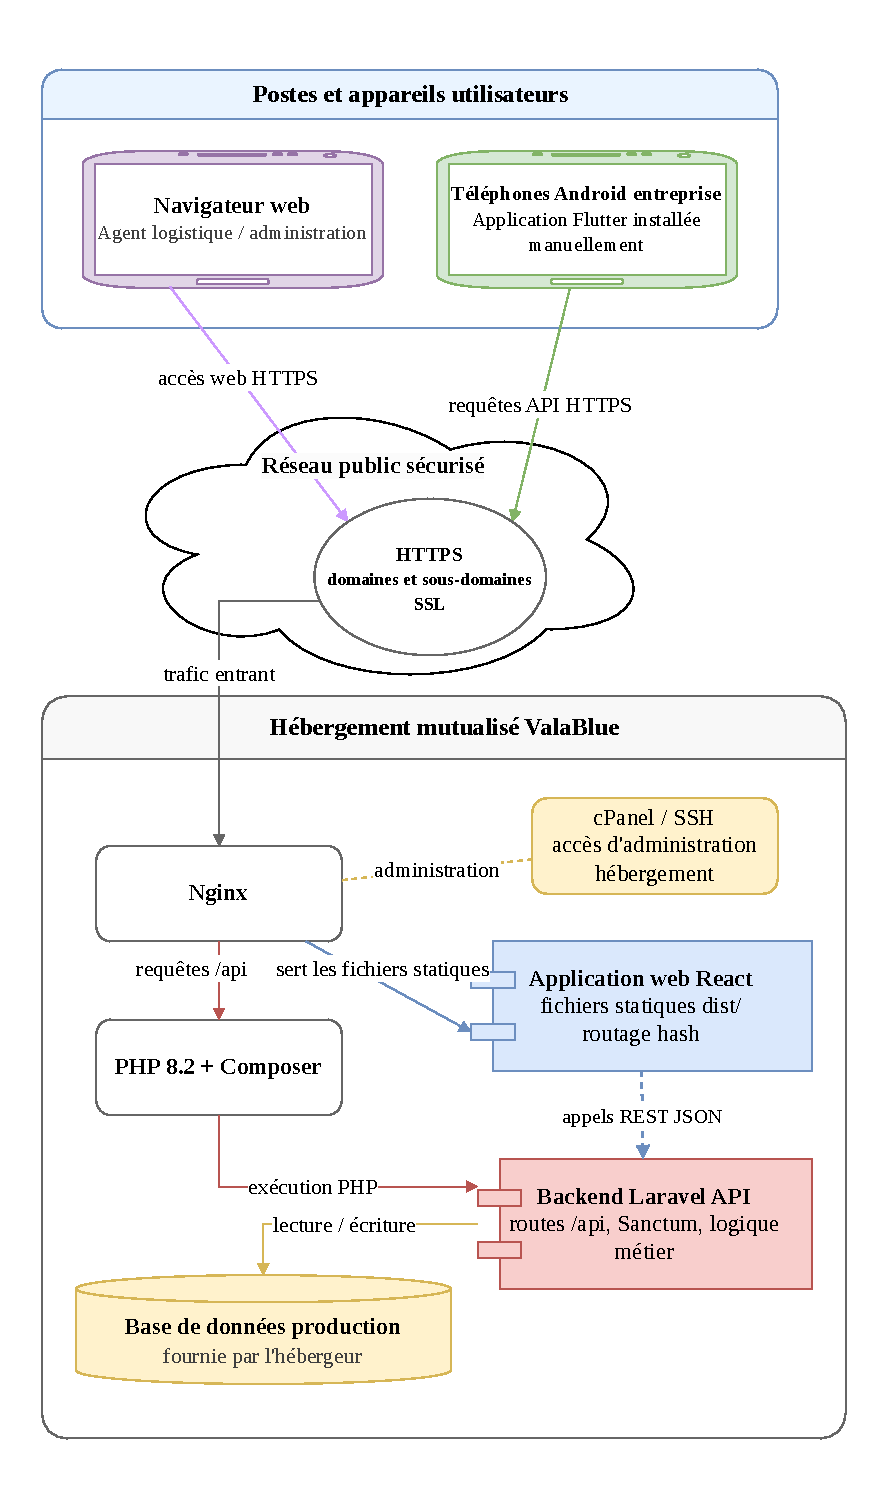
\includegraphics[width=\textwidth,height=0.92\textheight, keepaspectratio]
    {figures/architecture/diagramme-deploiement.pdf}

    \caption{Diagramme de déploiement UML de SomaScan}

    \label{fig:diagramme-deploiement-uml}
\end{figure}

\section{Processus de déploiement}

Le déploiement de SomaScan est organisé autour de GitHub et de pipelines automatisés. L'ensemble du code source est hébergé au sein d'une organisation GitHub dédiée, qui regroupe les trois dépôts du projet :

\begin{itemize}
    \item \texttt{somascan-be} : le backend Laravel ;
    \item \texttt{somascan-admin-fe} : l'application web React destinée à l'administration ;
    \item \texttt{somascan-operator-fe} : l'application mobile Flutter pour les opérateurs terrain.
\end{itemize}

Cette organisation centralisée permet de gérer les accès, les secrets et les workflows GitHub Actions de manière cohérente pour l'ensemble de la solution. La branche \texttt{master} de chaque dépôt représente l'état stable du code source et est directement connectée à l'environnement de production. Par conséquent, toute modification fusionnée dans cette branche peut avoir un impact direct sur la version utilisée en production.

Pour limiter ce risque, la branche \texttt{master} est protégée et ne doit pas recevoir de push direct. Les modifications sont développées dans des branches dédiées, puis intégrées à travers des Pull Requests après validation.

Le processus général de livraison suit les étapes suivantes :

\begin{enumerate}
    \item créer une branche dédiée pour la fonctionnalité, la correction ou la modification ;
    \item implémenter et tester les changements dans cette branche ;
    \item ouvrir une Pull Request vers la branche \texttt{master} ;
    \item relire, valider et approuver les changements ;
    \item fusionner la Pull Request dans \texttt{master} ;
    \item déclencher automatiquement le déploiement de la nouvelle version en production.
\end{enumerate}

\begin{figure}[H]
    \centering
    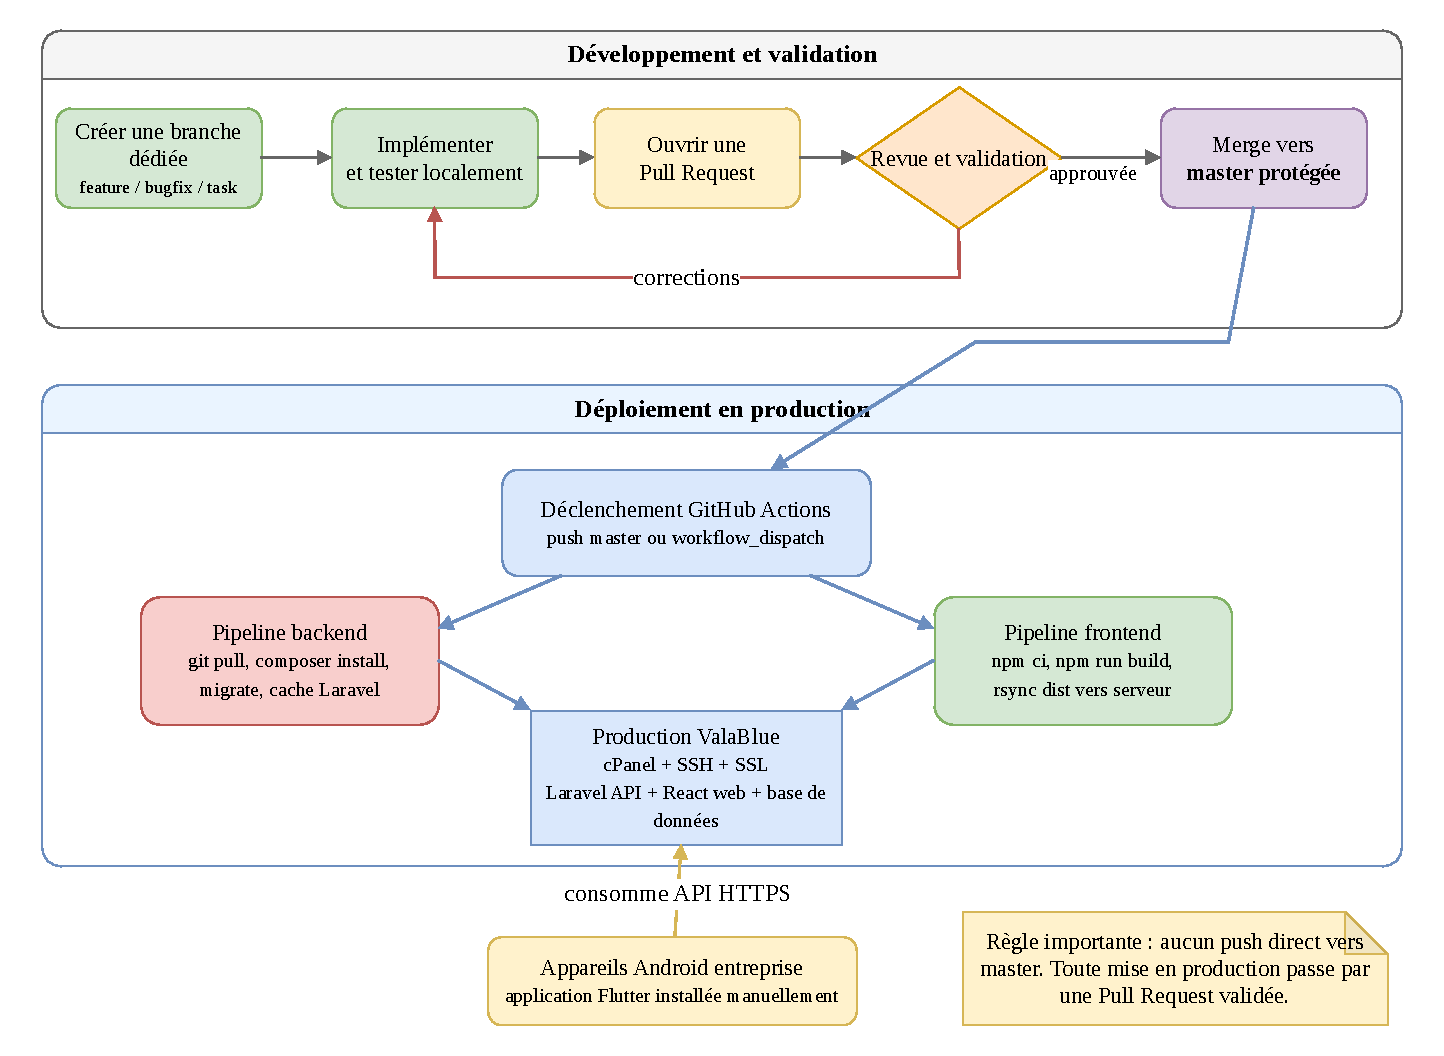
\includegraphics[width=\textwidth,keepaspectratio]
    {figures/diagrams/processus-deploiement.pdf}

    \caption{Processus de déploiement de SomaScan}

    \label{fig:processus-deploiement}
\end{figure}

\subsection*{Déploiement du backend Laravel}

Le déploiement du backend est automatisé par le fichier \codepath{.github/workflows/deploy.yaml}. Ce pipeline peut être déclenché de deux manières : automatiquement lors d'un push sur la branche \texttt{master}, ou manuellement avec l'action \path{workflow_dispatch} en précisant la branche à déployer.

Le pipeline backend exécute les opérations principales suivantes :

\begin{enumerate}
    \item récupérer le code source depuis GitHub ;
    \item charger la clé SSH stockée dans les secrets GitHub ;
    \item ajouter le serveur de production aux hôtes connus SSH ;
    \item se connecter au serveur et mettre à jour le code avec \texttt{git fetch}, \texttt{git checkout} et \texttt{git pull};
    \item installer les dépendances PHP avec Composer en mode production ;
    \item nettoyer l'optimisation Laravel ;
    \item exécuter les migrations avec l'option \texttt{--force} ;
    \item mettre en cache la configuration et les routes ;
    \item redémarrer les workers de queue si des processus sont actifs.
\end{enumerate}

Cette automatisation réduit les erreurs liées aux manipulations manuelles et garantit que chaque déploiement suit les mêmes étapes. L'utilisation des secrets GitHub permet de ne pas exposer les informations sensibles comme l'hôte SSH, l'utilisateur, le port, la clé privée ou le chemin de déploiement.

\subsection*{Déploiement de l'application web React}

Le déploiement du frontend est automatisé par le fichier \codepath{.github/workflows/frontend-deploy.yaml}. Comme pour le backend, ce pipeline se déclenche automatiquement lors d'un push sur \texttt{master} ou manuellement avec un choix de branche.

Le pipeline frontend suit les étapes suivantes :

\begin{enumerate}
    \item récupérer le code source de la branche à déployer ;
    \item installer Node.js en version 22 ;
    \item installer les dépendances avec \texttt{npm ci} ;
    \item compiler l'application avec \texttt{npm run build} ;
    \item charger la clé SSH depuis les secrets GitHub ;
    \item vérifier l'accès au dossier de déploiement distant ;
    \item synchroniser le dossier \codepath{dist/} vers le serveur avec \texttt{rsync};
    \item supprimer les anciens fichiers qui ne sont plus présents dans la nouvelle version grâce à l'option \texttt{--delete}.
\end{enumerate}

Ce processus permet de déployer uniquement les fichiers statiques nécessaires au fonctionnement de l'application web. L'utilisation de \texttt{rsync} rend la synchronisation plus efficace et maintient le dossier de production cohérent avec le dernier build validé.

\subsection*{Distribution de l'application mobile}

L'application Flutter n'est pas publiée sur une plateforme publique. Elle est installée manuellement sur les téléphones Android fournis et administrés par l'entreprise. Ces appareils sont configurés pour exécuter cette application métier dédiée.

Ce mode de distribution est adapté au contexte du projet, car les utilisateurs de l'application mobile sont limités aux opérateurs terrain autorisés. Il facilite également le contrôle des appareils utilisés pour les scans, tout en évitant une exposition inutile de l'application sur un store public.

\section{Workflow DevOps et pipeline CI/CD}

Le workflow DevOps adopté repose sur une séparation claire entre le développement, la validation et la production. Les développeurs travaillent sur des branches isolées, puis proposent leurs changements à travers des Pull Requests. La branche \texttt{master} conserve uniquement le code validé et prêt à être livré.

\begin{figure}[H]
    \centering
    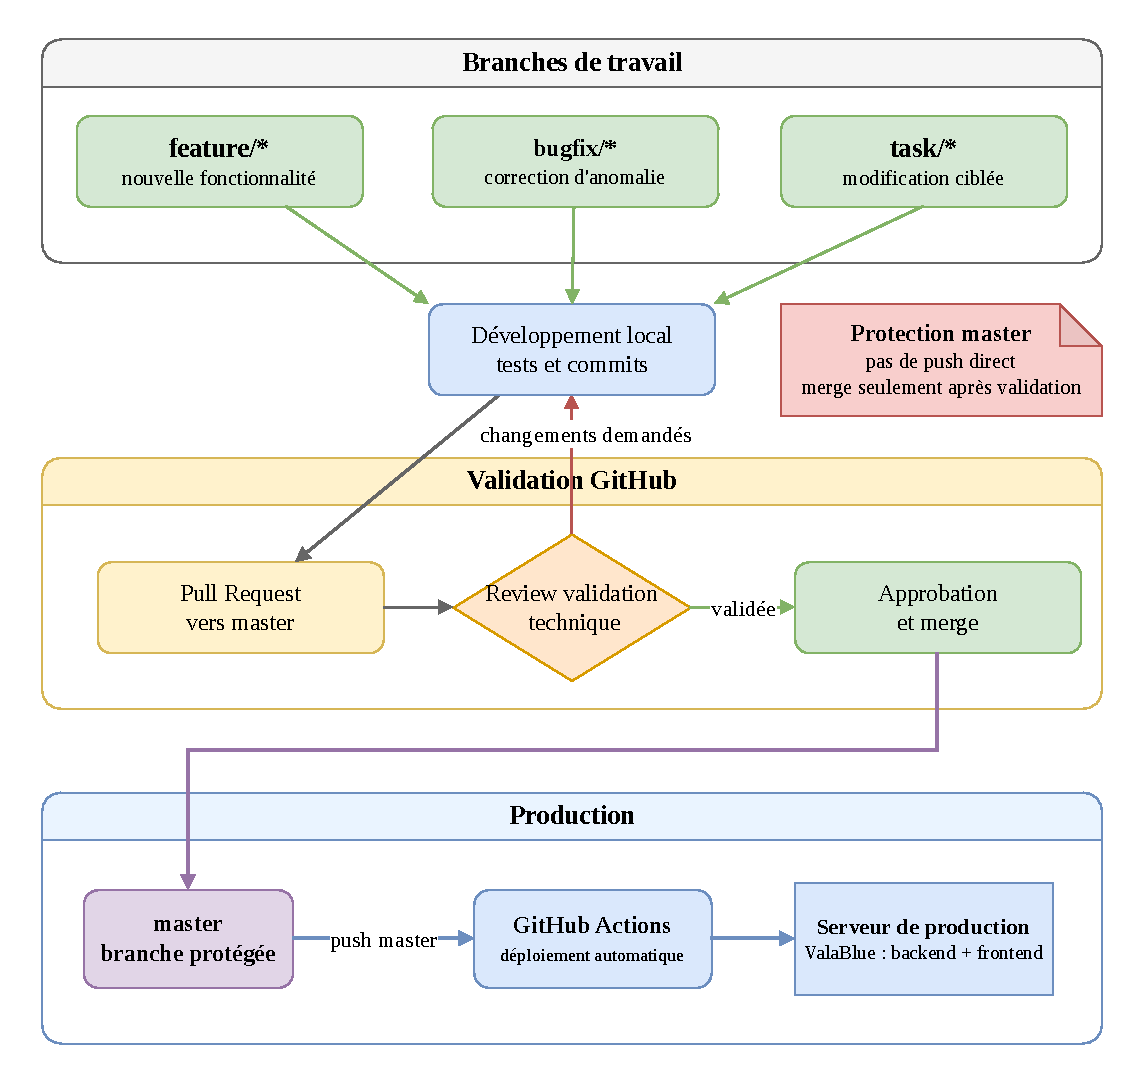
\includegraphics[width=\textwidth,keepaspectratio]
    {figures/diagrams/workflow-git.pdf}

    \caption{Workflow Git de développement, validation et production}

    \label{fig:workflow-git}
\end{figure}

Les pipelines CI/CD assurent ensuite la continuité entre la validation du code et le déploiement. Dans le cas de SomaScan, les workflows GitHub Actions jouent principalement le rôle de pipelines de déploiement continu. Ils automatisent la mise à jour du serveur, l'installation des dépendances, la compilation du frontend et les commandes post-déploiement nécessaires.

Le tableau~\ref{tab:pipelines-cicd} compare les deux pipelines utilisés.

\begin{table}[H]
\centering
\begin{tabularx}{\textwidth}{|p{3.5cm}|X|X|}
\hline
\textbf{Pipeline} & \textbf{Déclenchement} & \textbf{Actions principales} \\
\hline
Backend Laravel & Push sur \texttt{master} ou déclenchement manuel & Mise à jour du code sur le serveur, installation Composer, migrations, nettoyage et mise en cache Laravel. \\
\hline
Frontend React & Push sur \texttt{master} ou déclenchement manuel & Installation Node.js, installation des dépendances, build React, synchronisation du dossier \texttt{dist/} vers le serveur. \\
\hline
\end{tabularx}
\caption{Pipelines CI/CD utilisés pour SomaScan}
\label{tab:pipelines-cicd}
\end{table}

\begin{figure}[H]
    \centering
    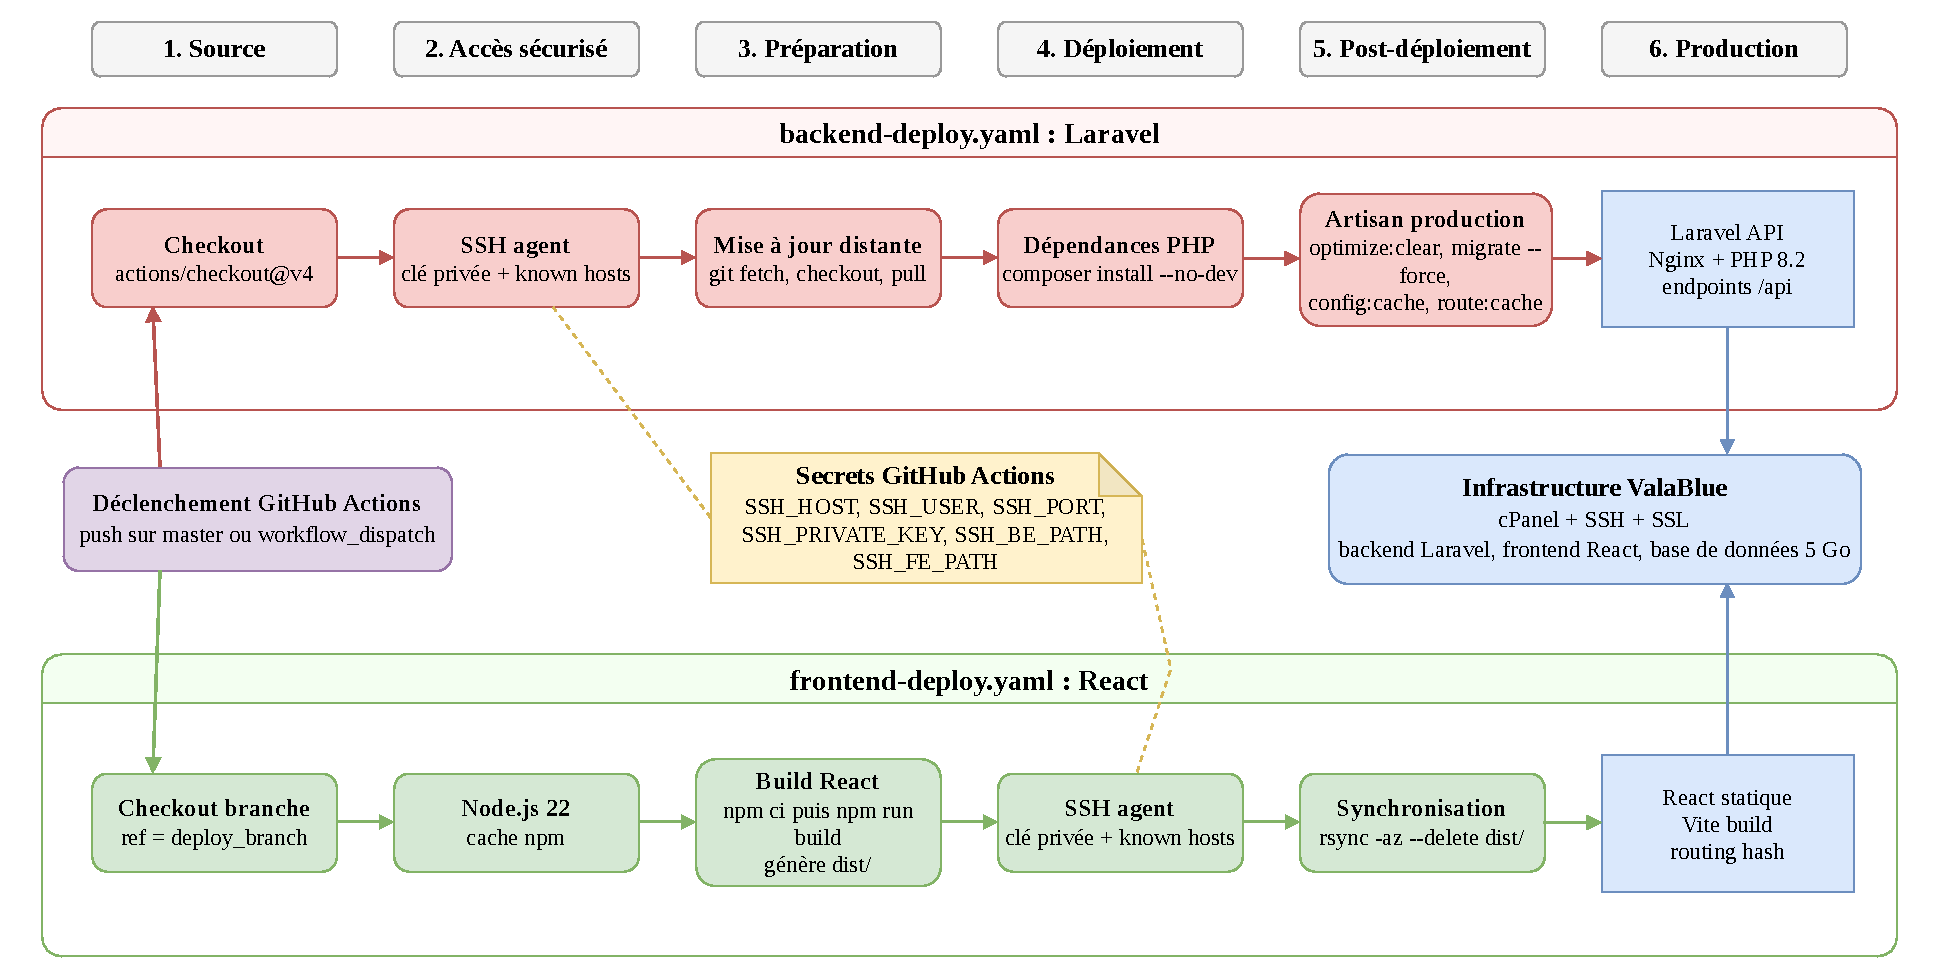
\includegraphics[width=\textwidth,keepaspectratio]
    {figures/diagrams/pipeline-ci-cd.pdf}

    \caption{Pipeline CI/CD backend et frontend}

    \label{fig:pipeline-ci-cd}
\end{figure}

Les variables sensibles nécessaires au déploiement sont stockées dans les secrets GitHub. Cette pratique évite de placer des identifiants ou des chemins sensibles directement dans le code source. Les principaux secrets concernent notamment le serveur SSH, l'utilisateur SSH, le port SSH, la clé privée, le chemin du backend et le chemin de déploiement du frontend.

\section{Sécurité et limites opérationnelles actuelles}

La sécurité de production repose d'abord sur l'utilisation de certificats SSL valides pour les domaines et sous-domaines de production. Les échanges entre les applications clientes et le backend sont donc protégés par HTTPS. Du côté applicatif, l'authentification repose sur les jetons gérés par Laravel Sanctum, tandis que les autorisations sont contrôlées par les rôles définis dans l'application.

Les accès de déploiement reposent sur SSH et sur les secrets GitHub Actions. Cette séparation permet de ne pas exposer directement les identifiants dans le dépôt. L'accès à la branche \texttt{master} doit rester strictement contrôlé, car cette branche déclenche les déploiements vers la production.

À ce stade, aucun dispositif dédié de supervision applicative n'est encore mis en place. Il n'existe pas non plus de processus formalisé de maintenance préventive. Les seules traces directement exploitables sont les résultats des pipelines GitHub Actions, les erreurs éventuellement observées dans l'environnement d'hébergement et les retours fonctionnels des utilisateurs. Il est donc préférable de présenter cette partie comme une limite opérationnelle actuelle plutôt que comme une fonctionnalité déjà réalisée.

Une limite importante de l'état actuel concerne la sauvegarde de la base de données. Aucune stratégie de sauvegarde automatisée n'est encore mise en place. Pour une exploitation durable, il est recommandé de mettre en place au minimum une sauvegarde régulière de la base de données, par exemple sous forme d'exports SQL planifiés ou de sauvegardes fournies par l'hébergeur. Cette amélioration réduira le risque de perte de données en cas d'erreur humaine, de problème serveur ou de migration incorrecte.

\section{Bénéfices et limites du déploiement}

L'organisation actuelle du déploiement présente plusieurs bénéfices. L'utilisation d'une seule infrastructure pour le backend, le frontend et la base de données simplifie l'administration. Le mode hash du routage React facilite l'hébergement de l'application web sur une plateforme mutualisée. Les pipelines GitHub Actions réduisent les manipulations manuelles et rendent le processus de livraison plus répétable. Enfin, la protection de la branche \texttt{master} impose un passage par Pull Request avant toute mise en production.

Cependant, certaines limites doivent être prises en compte. L'hébergement mutualisé offre moins de contrôle qu'un serveur dédié ou un VPS. L'absence de sauvegarde automatique de la base de données constitue un risque opérationnel. De plus, comme la branche \texttt{master} est reliée directement à la production, toute erreur fusionnée dans cette branche peut être rapidement propagée. Il est donc nécessaire de maintenir une validation rigoureuse avant chaque merge.

En cas d'incident après un déploiement, la stratégie de retour arrière la plus simple consiste à restaurer une version précédente du code depuis Git, puis à relancer le pipeline ou à remettre à jour le serveur par SSH. Pour la base de données, cette stratégie reste incomplète tant qu'une politique de sauvegarde n'est pas mise en place.

\section{Conclusion}

Ce chapitre a présenté l'environnement de production et les pratiques DevOps utilisées pour SomaScan. La solution est hébergée sur une infrastructure ValaBlue administrée via cPanel et SSH. Le backend Laravel, l'application web React et la base de données sont regroupés sur la même plateforme, tandis que l'application mobile Flutter est installée manuellement sur les appareils Android de l'entreprise.

Le déploiement repose sur GitHub Actions, avec deux pipelines distincts pour le backend et le frontend. La branche \texttt{master} est protégée et sert de point d'entrée vers la production après validation par Pull Request. Cette organisation permet d'obtenir un processus de livraison plus fiable, plus traçable et moins dépendant des opérations manuelles.

La principale amélioration à prévoir concerne la mise en place d'une stratégie de sauvegarde de la base de données. À terme, l'ajout d'une supervision applicative et d'un processus de maintenance formalisé pourrait renforcer la robustesse opérationnelle de SomaScan et préparer son évolution vers une exploitation plus mature.
